\chapter{Einführung in Google Fusion Tables}

\section{SQL API}
Das SQL API bietet eine REST-Schnittstelle mit welcher man mit SQL-ähnlichen Befehlen Daten aus Google Fusion Tables abfragen oder verändern kann. Sie verfügt bereits über eine grosse Palette an möglichen Befehlen.

\begin{tabular}{|l|l|}
\hline 
Befehl & Beschreibung \\ 
\hline 
SHOW TABLES & Abfrage aller Tabellen des angemeldeten Benutzers \\ 
\hline 
DESCRIBE & Bezeichnung und Datentypen aller Spalten in einer Tabelle \\ 
\hline 
CREATE TABLE & Erstellen einer neuen Tabelle \\ 
\hline 
CREATE VIEW & Erstellen einer View auf Grundlage einer bestehenden Tabelle \\ 
\hline 
SELECT & Selektieren von Daten einer Tabelle \\ 
\hline 
INSERT & Neue Zeile zu einer Tabelle hinzufügen \\ 
\hline 
UPDATE & Daten in einer Tabelle verändern \\ 
\hline 
DELETE & Daten aus einer Tabelle löschen \\ 
\hline 
DROP TABLE & Löschen einer Tabelle \\ 
\hline 
\end{tabular}

\subsection{Client Libraries}
Google bietet zum API bereits auch Client Libraries in den Sprachen PHP und Phyton an. Da unserer Applikation aber möglichst nur in Javascript implementiert werden soll erstellten wir uns eine Javascript Library zur Verwendung des SQL APIs.

Durch die Same origin policy\footnote{Die Same-Origin-Policy (SOP) ist ein Sicherheitskonzept, das es JavaScript und ActionScript nur dann erlaubt, auf Objekte einer anderen Webseite zuzugreifen, wenn sie aus derselben Quelle (Origin) stammen.\cite{sop} }, welche es uns daran hinderte AJAX-Requests direkt auf das Google API abzusetzen, mussten wir zuerst nach Lösungen für dieses Problem suchen. Wir wollten es verhindern einen PHP-Server dazwischen zu schalten, welcher uns die Abfragen abnimmt.

So fanden wir in den Google Groups ein inoffizielles JSONP API, welches es erlaubt AJAX-Requests auch über die eigene Domäne hinweg zu senden.

\section{Geocodierung}
Ein grosser Vorteil der Google Fusion Tables ist die automatische 
\gls{Geocodierung} von Standortdaten. Sobald eine neue Zeile zu einer Tabelle hinzugefügt wird, werden alle Zellen vom Typ \emph{Location} einem eindeutigen Standort auf der Karte zugewiesen. Ist dies nicht möglich, da beispielsweise eine Adresse in mehreren Orten vorkommen kann, bleibt die Zelle gelb hinterlegt.
 
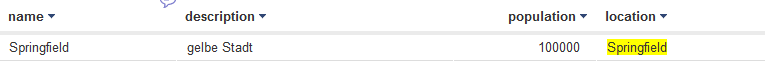
\includegraphics[scale=0.75]{images/geocoding_failed.png}

Diese geocodierten Standorte werden in der Tabelle hinterlegt sind aber mit den SQL API nicht selektierbar. Man müsste also für jede Zeile die man als Resultat erhält die Geocodierung manuell vornehmen, was sich negativ auf die Ladezeit der Karte auswirken würde.
Es gibt verschiedene Dienste, welche eine solche Geocodierung von Standortdaten anbieten. Die meisten davon haben aber eine Begrenzung der möglichen Anfragen pro Tag.

\begin{tabular}{|l|p{1.9cm}|p{7.3cm}|}
\hline 
Anbieter & Anfragen pro Tag & URL \\ 
\hline 
Google Maps Geocoding API & 2500 & \url{https://developers.google.com/maps/documentation/geocoding/?hl=de} \\ 
\hline 
Yahoo! PlaceFinder API & 50000 & \url{http://developer.yahoo.com/geo/placefinder/} \\ 
\hline 
MapQuest Geocoding API & keine Begrenzung & \url{http://developer.mapquest.com/web/products/dev-services/geocoding-ws} \\ 
\hline 
\end{tabular} 

Wie man sieht erreicht man mit diesen Diensten beim Arbeiten mit grossen Datenmengen schnell die Grenzen.

\section{Google Maps API - FusionTablesLayer}
Google bietet von Haus aus aber bereits eine Fusion Table-Integration im Google Maps API V3 an. Damit ist es möglich Fusion Tables als eigenständige Layer direkt auf der Karte darzustellen.
Die Möglichkeiten dieser Layer sind noch stark eingeschränkt aber die grundlegenden Funktionalitäten für das Arbeiten mit Geodaten sind bereits vorhanden.

So ist es möglich Abfragen mit WHERE-Conditions einzuschränken oder die Stile des Layers selbst zu bestimmen. Man kann beispielsweise Flächen mit Zeckengebieten je nach Intensität des Befalls anders einfärben.

\subsection{Spatial-Queries}
Zudem bieten die FusionTablesLayer bereits eine Reihe von speziellen ortsabhängigen Abfrage-Möglichkeiten.

\begin{tabular}{|p{4cm}|p{11cm}|}
\hline 
Spatial Keyword & Beschreibung \\ 
\hline 
ST{\_}INTERSECTS( {\textless}location{\_}column{\textgreater}, {\textless}geometry{\textgreater} ) & Kann als Bedingung in der WHERE-Klausel des Statements verwendet werden.

Liefert alle Zeilen zurück, welche sich innerhalb der definierten Geometrie \emph{{\textless}geometry{\textgreater}} befinden.

\begin{itemize}
\item Als \emph{{\textless}location{\_}column{\textgreater}} muss eine Spalte der Tabelle angegeben werden, welche den Typ \emph{location} hat.
\item Als \emph{{\textless}geometry{\textgreater}} kann entweder ein \emph{CIRCLE} oder ein \emph{RECTANGLE} verwendet werden. 
\end{itemize}

\textit{Hinweis: ST{\_}INTERSECTS und ST{\_}DISTANCE dürfen nicht zusammen im gleichen Statement verwendet werden.} \\ 
\hline 
ST{\_}DISTANCE( {\textless}location{\_}column{\textgreater}, {\textless}coordinate{\textgreater} ) & Kann als Bedingung in der ORDER BY-Klausel des Statements verwendet werden.

Liefert die Datensätze sortiert nach der Distanz zur angegebenen Koordinate \emph{{\textless}coordinate{\textgreater}} zurück.

\begin{itemize}
\item Als \emph{{\textless}location{\_}column{\textgreater}} muss eine Spalte der Tabelle angegeben werden, welche den Typ \emph{location} hat.
\item Die \emph{{\textless}coordinate{\textgreater}} stellt die Koordinate dar, zu welcher der Abstand gemessen werden soll. 
\end{itemize}

\textit{Hinweis: ST{\_}INTERSECTS und ST{\_}DISTANCE dürfen nicht zusammen im gleichen Statement verwendet werden.} \\ 
\hline 
CIRCLE( {\textless}coordinate{\textgreater}, {\textless}radius{\textgreater} ) & Wird verwendet, um einen Kreis von der angegebenen Koordinate \emph{coordinate} mit den Radius \emph{radius} zu erhalten. \\ 
\hline 
POLYGON( {\textless}coordinate{\_}1{\textgreater}, {\textless}coordinate{\_}2{\textgreater}, ... ) & Wird verwendet um ein Polygon bestehend aus den angegebenen Koordinaten \emph{coordinate{\_}x} zu erhalten. \\ 
\hline 
RECTANGLE( {\textless}coordinate{\_}1{\textgreater}, {\textless}coordinate{\_}2{\textgreater} ) & Wird verwendet um ein Rechteck mit den Ecken \emph{coordinate{\_}1} (links oben) und \emph{coordinate{\_}2} (rechts unten) zu erhalten. \\ 
\hline 
\end{tabular} 

\subsection{Karten-Stile}
Die FusionTablesLayer bieten ein abfragebasiertes Styling der Ebene an. Damit ist es möglich Flächen oder Linien farblich hervorzuheben oder Custom-Icons für Markierung zu verwenden. Zu jedem Stil kann man eine Einschränkung festlegen, welche bestimmt, ob dieser für den aktuellen Datensatz angewendet wird oder nicht. Damit ist es möglich die Ebene stark zu personalisieren.

\subsubsection{Beispiel eines Stils:}
\lstset{language=HTML}
\begin{lstlisting}
styles: [{
	polygonOptions: {
		fillColor: "#00FF00", // gruen
		fillOpacity: 0.3
	}
}, {
	where: "birds > 300",
	polygonOptions: {
		fillColor: "#0000FF" // blau
	}
}]
\end{lstlisting}

In diesem Beispiel werden alle Polygone der Tabelle, welche in der Spalte \emph{birds} eine Zahl grösser als 300 eingetragen haben, \emph{blau} eingefärbt. Die restlichen Polygone erhalten eine \emph{grüne} Färbung mit einer Deckkraft von 30\%.

\subsubsection{Einschränkungen}
Das Google Maps API hat momentan folgende Einschränkungen bezüglich den Ebenenstilen definiert.

\begin{itemize}
\item Auf einer Karte können maximal 5 FusionTablesLayer gleichzeitig angezeigt werden
\item Stile können dabei nur für eine dieser Ebenen angewendet werden
\item Zudem dürfen für diese Ebene maximal 5 Stile definiert sein
\end{itemize}

\subsection{Heatmaps}
Ein weiteres mächtiges Feature ist zudem die Möglichkeit die Daten der Tabelle direkt als Heatmap darzustellen. Dabei werden die Daten automatisch nach der Häufigkeit der Vorkommnisse an einem Ort anders eingefärbt. Der verwendete Farbverlauf geht dabei von Grün (für wenig Daten) bis Rot (für viele Daten). 

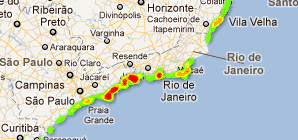
\includegraphics{images/gmap_fusiontableslayer_heatmap.png}

\subsection{Vorteil}
Der grösste Vorteil der Fusion Table-Ebenen findet man aber eher darin, dass die Geocodierung der Standort-Daten direkt aus der Tabelle gelesen wird und nicht manuell abgefragt werden muss. Dadurch kann die Ebene komplett auf den Servern von Google aufbereitet werden. Der Client muss die erhaltenen Daten lediglich noch darstellen. Der Vorteil davon wird durch das folgende Diagramm schnell ersichtlich.

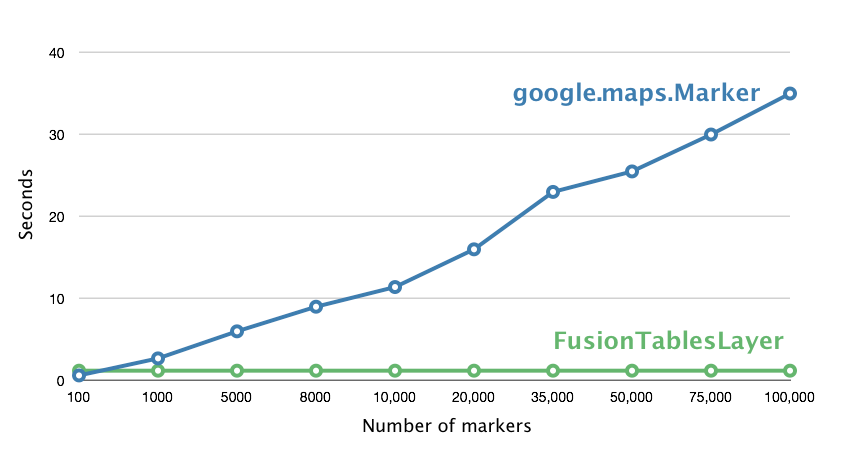
\includegraphics[scale=0.5]{images/gmap_fusiontableslayer_vs_markers.png}

Die Zeit für das Rendering der Karte bleibt demnach bei der Verwendung von Fusion Table-Ebenen konstant und somit unabhängig von der Anzahl Markierungen, welche gesetzt werden müssen. Der Rechenaufwand, der für das Erstellen der Javascript Marker-Objekte verwendet werden müsste, wird direkt von den Google Servern übernommen und das Resultat als Bild zum Client gesendet. Daraus resultiert die konstante Zeit, welche für die Anfrage zum Server und für das Senden der Antwort zum Client verwendet wird.

\subsection{Nachteil}
Ein grosser Nachteil dieser Fusion Table-Ebenen besteht aber darin, dass die verwendeten Fusion Tables als  \emph{öffentlich} markiert sein müssen. Sprich jeder kann die Tabellen anzeigen oder auslesen. Es ist also nicht möglich eine Tabelle mit sensiblen Daten als Fusion Table-Ebene darzustellen.

Von Google wird zur Lösung dieses Problems aber folgendes Vorgehen vorgeschlagen: Man kann für Tabellen mit sensiblen Inhalten eine View erstellen, welche lediglich die öffentlichen Spalten und Zeilen selektiert. Diese View könnte man dann als \emph{öffentlich} markieren und in einer Fusion Table-Ebene verwenden.

Es bleibt die Frage offen, wie es möglich ist sensible Daten trotzdem in eine Ebene einzubringen.

\subsection{Einschränkungen}
Einige Einschränkungen sind aber auch bei der Verwendung der Fusion Tables-Ebenen zu beachten. Wie bereits erwähnt ist es nur möglich \emph{öffentliche} Fusion Tables als FusionTablesLayer darzustellen.

Zusätzlich ist die Anzahl an Markierungen, die auf einer Fusion Table-Ebene angezeigt werden können, auf 100000 Stück beschränkt. Diese Zahl sollte grundsätzlich aber für die meisten Anwendungsfälle gut ausreichen.

Bei einer grösseren Anzahl von Daten sollte man sich bezüglich Übersicht zuerst die Überlegung machen, ob es Sinn macht alle Markierungen auf einmal darzustellen. Man könnte beispielsweise nur die Daten in einem gegebenen Umkreis darstellen. Auch die Performance nimmt bei einer grossen Anzahl von Markierungen schnell ab.

\section{Google Fusion Table Javascript Library (gftlib-js)}
Die Google Fusion Table Javascript Library vereinfacht die Kommunikation mit dem Google Fusion Table SQL API. Sie hilft dabei SQL-Queries zu erstellen und per AJAX an das API zu versenden.

Zur Erstellung der AJAX-Requests werden die \$.get()- und \$.post()-Helpermethoden der jQuery Library in der Version 1.7.1 (Minified) verwendet.

\subsection{Abhängikeiten}
\begin{tabular}{|l|l|}
\hline 
Library & Version \\ 
\hline 
jQuery & 1.7.1-min \\ 
\hline 
\end{tabular} 

\subsection{Methoden}
\begin{tabular}{|l|p{5cm}|p{5cm}|}
\hline 
Methode & Beschreibung & Parameter \\ 
\hline 
execSql(callback, query) & Führt einen SQL-Befehl & callback (Funktion): Callback-Methode welche nach Beendigung der Methode aufgerufen wird. query (String): SQL-Query \\ 
\hline 
execSelect(callback, options) & Führt einen SQL-Abfrage aus & callback (Funktion): Callback-Methode welche nach Beendigung der Methode aufgerufen wird. query (String): SQL-Query \\ 
\hline 
convertToObject(gftData) & Konvertiert das Resultat einer Abfrage in sprechende Objekte & • \\ 
\hline 
\end{tabular} 
